\documentclass[a4paper, apacite, 12pt, doc]{apa6}

\usepackage[utf8]{inputenc}
\usepackage[spanish]{babel}
\usepackage{apacite, hyperref, amsmath, listings, graphicx}

\graphicspath{ {./images/} }
% \usepackage[backend=biber, sytle=apa]{biblatex}
% \addbibresource{biblio.bib}
\usepackage{mathtools}
\usepackage{systeme}

\title{ Taller 1: Sistemas de Ecuaciones Lineales y No Lineales}
\shorttitle{ Doctorado en Tecnologías de la Información y la Comunicación}
\author{Eugenia Arrieta Rodríguez}
\affiliation{Universidad de la Costa}



\begin{document}

\maketitle

\section{Pregunta 1:  Será sencillo representar cualquier sistema de dos por dos? ¿Cómo se representarán sistemas de tres ecuaciones con tres incógnitas?}


Un sistema de  ecuaciones lineales con dos incógnitas se puede interpretar graficamente como dos rectas en el plano cartesiano:


\begin{figure}[h]
	\centering
	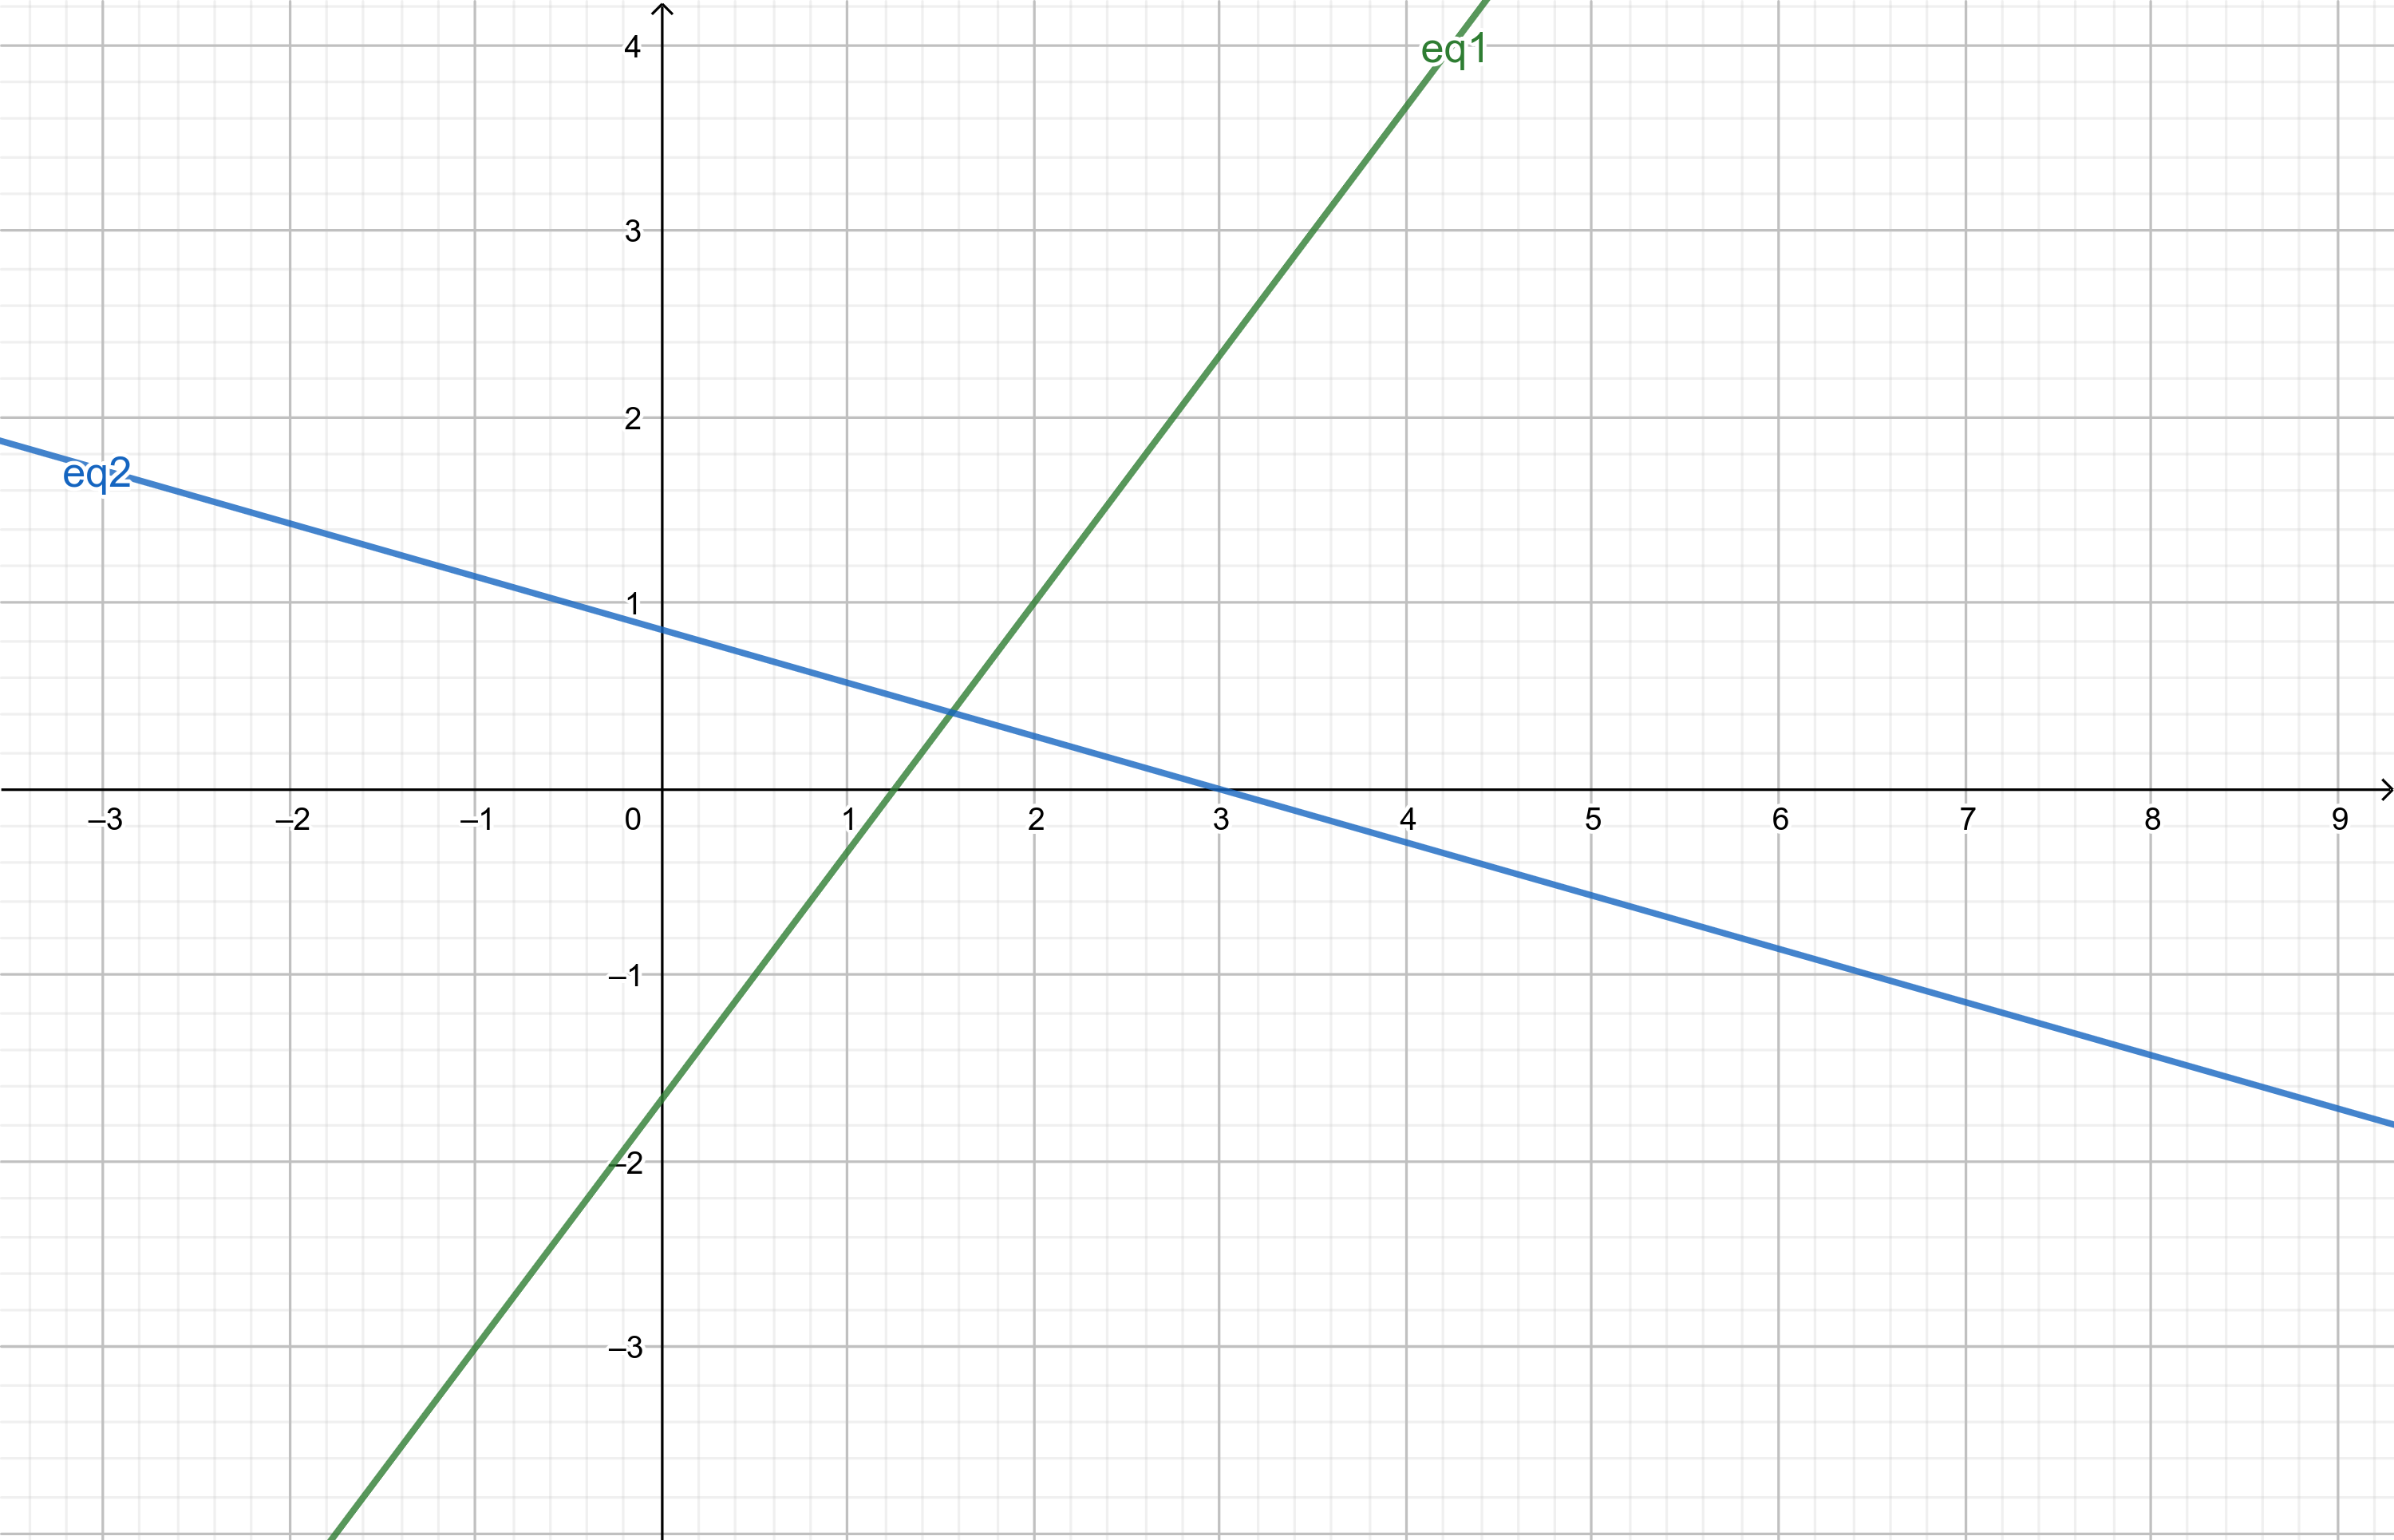
\includegraphics[scale=0.9]{img01}
	\caption{Representación gráfica de un sistema lineal 2x2}
\end{figure}

La \textit{Figura 1} puede ser expresada completamente por un sistema de ecuaciones, de la siguiente manera:

\[
\systeme*{4x -3y = 5, 2x + 7y = 6}
\]

Cada una de las ecuaciones anteriores representan una recta en el plano de la figura 1. Para este caso el sistema de ecuaciones tiene solución y será el punto de corte de ambas rectas. Solucionar un sistema de ecuaciones es encontrar los valores de de las incógnitas (para este caso: $x$, $y$) que hacen cumplir todas igualdades.

 Puede que un sistema de 2 ecuaciones con 2 incógnitas tenga o no solucion, se pueden presentar los siguientes casos:

\begin{itemize}
	\item  Que no tenga ninguna solución. Se denomina “sistema incompatible”. Las dos ecuaciones representan a dos rectas paralelas y que por tanto no existe ninguna combinación de las incógnitas que satisfaga las igualdades.

\begin{figure}[h]
	\centering
	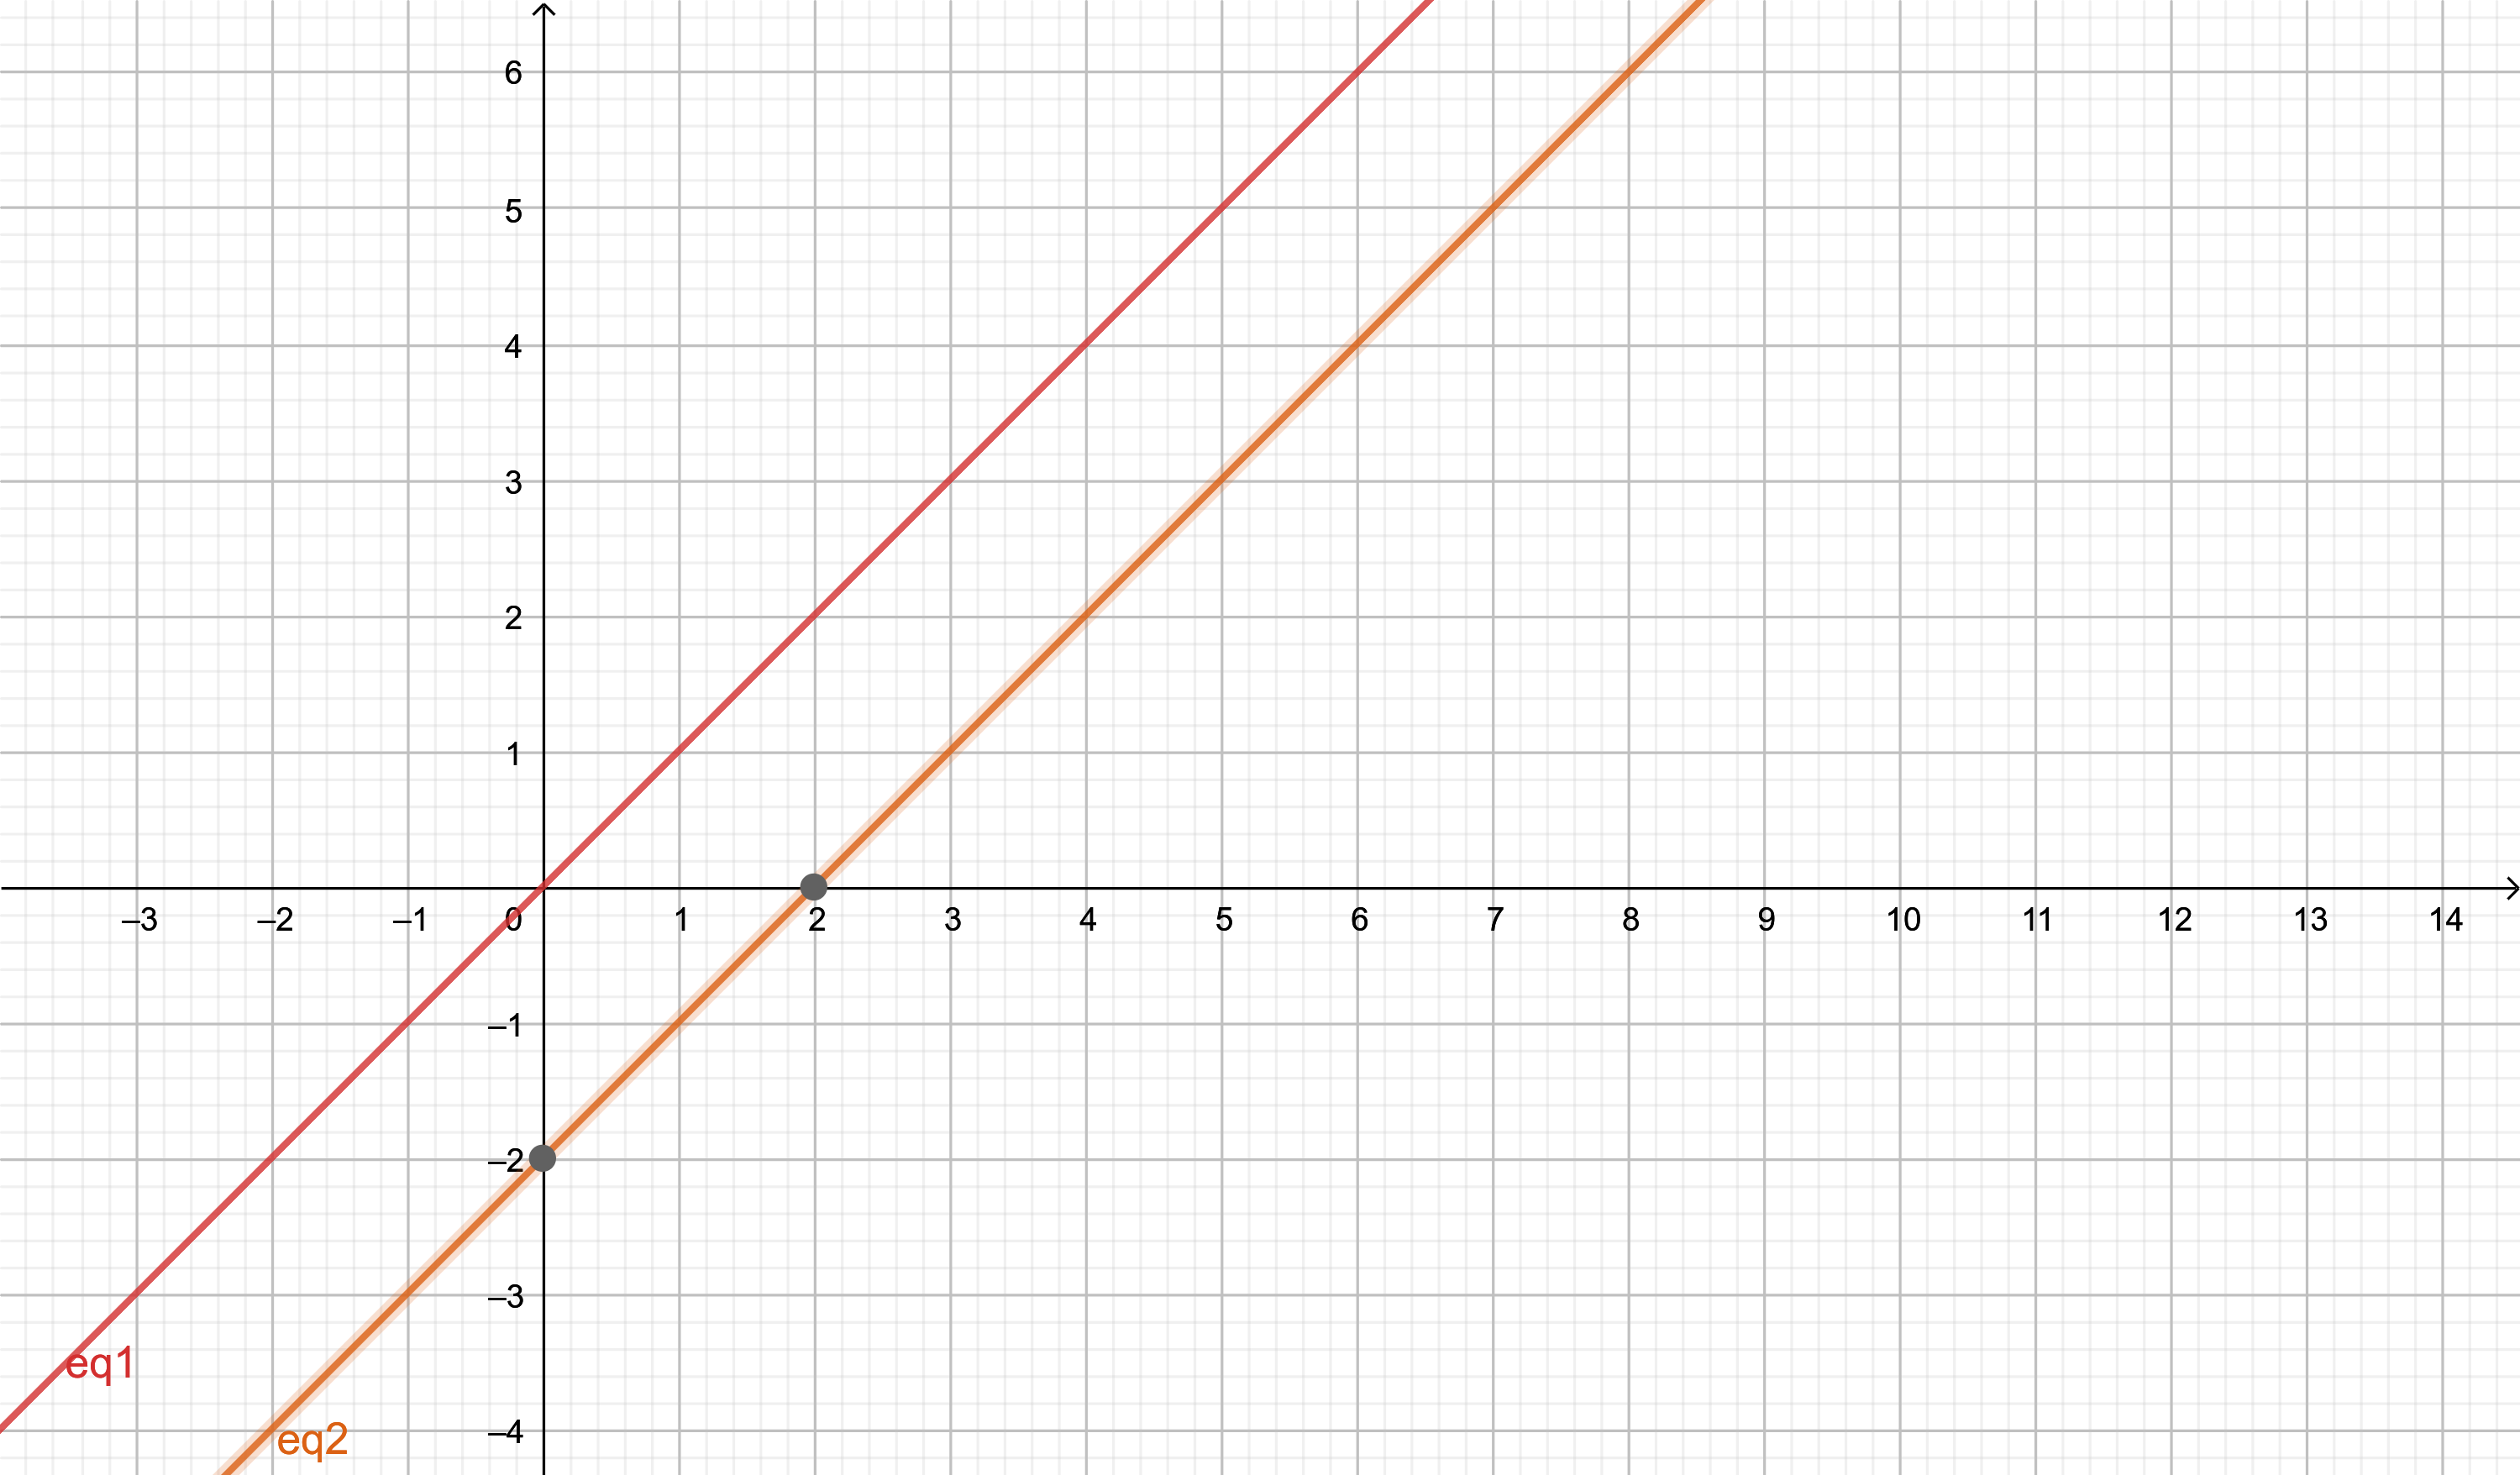
\includegraphics[scale=0.75]{img02}
	\caption{Representación gráfica de un sistema lineal 2x2 que no tiene solución}
\end{figure}



\item Que tenga infinitas soluciones. Se denomina “sistema compatible indeterminado”. Las dos ecuaciones representan a dos rectas superpuestas, una encima de otra (coinciden en todos los puntos)




\item Que tenga una única solución. Como en el ejemplo de la figura 1. Se denomina “sistema compatible determinado”. Las dos ecuaciones representan a dos rectas que se cortan en un solo punto

\end{itemize}


\subsection{Resolución de un sistema lineal de dos ecuaciones}

Existen varios métodos para resolver sistemas de ecuaciones lineales:

\begin{itemize}
	\item Método de sustitución.
	\item Método de igualación.
	\item Método de reducción.
	\item Método de Gauss.
	\item Regla de Cramer.
	\item Algoritmos numericos.
\end{itemize}

Los sistemas de ecuaciones lineales pueden tener más  dos variables. Las ecuaciones con una variable se representan en la recta de los reales. Las ecuaciones con dos variables se grafican en un plano. Las ecuaciones con tres variables se grafican en un espacio tridimensional. Las ecuaciones con una variable requieren sólo una ecuación para tener una solución única. Las ecuaciones con dos variables requieren dos ecuaciones para tener una solución única (un par ordenado). En general un sistema de $n$ variables necesita estar compuesto por $n$ ecuaciones para poder tener una solucion unica. Donde $n \in Z^+, n > 0$

Ejemplo: Sea un sistema de ecuaciones lineales 3x3:
\[
\systeme*{2x+3y+4z=20, 3x-5y-z= -10, -x+2y-3z =-6}
\]

Sea la ecuación (a) el resultado de multiplicar la ecuación (1) y la ecuación (2) por 3 y -2 respectivamente, luego operarlas:

\begin{center}
	\begin{tabular}{cccc}
		6x &+9y & +12z  & = 60 \\
		-6x &+9y & +2z  & = 20 \\
		\hline
		 0 & +19y & +14z & = 80
	\end{tabular}
\end{center}

Sea la ecuación (b) el resultado de multiplicar la ecuación (1) y la ecuación (3) por 1 y 2 respectivamente, luego operarlas:

\begin{center}
	\begin{tabular}{cccc}
		2x &+3y & +4z  & = 20 \\
		-2x &+4y & -6z  & = -6 \\
		\hline
		 0 & +7y & -2z & = 8
	\end{tabular}
\end{center}

Multiplicamos por 7 la ecuación (b) y la operamos con la ecuación (a)

\begin{center}
	\begin{tabular}{cccc}
		 & +19y & +14z & = 80 \\
		 & +49y & -14z & = 56 \\
		\hline
		&  +68y& 0  & = 136 \\
		&    y  &   & = $\frac{136}{68}$ \\
		&    y & &   = 2
	\end{tabular}
\end{center}

Inyectamos el valor encontrado de $y$ en la ecuacion (b):

\begin{gather*}
	7y -2z = 8 \\
	7(2) -2 = 3z = 8 \\
	z = \frac{8 - 14}{-2} \\
	z = \frac{6}{2} = 3
\end{gather*}


Inyectamos los valores encontrados de $y, z$ en la ecuacion (3):

\begin{gather*}
	-x+2y-3z =-6 \\
	-x +2(2) -3(3) = -6 \\
	-x = -6 -4 +9 \\
	x = \frac{-1}{-1} = 1
\end{gather*}



\begin{gather*}
\\
\\
\end{gather*}


\section{Pregunta 2: ¿Cuantas manos miden la anchura y el largo?}

Sea:

\[
\systeme*{\frac{1}{4}a +l = 7,
a +l = 10} \]

Multiplicamos por (-1) la ecuación (2), sumamos ambas ecuaciones para eliminar la variable $l$ y despejamos $a$:

\begin{gather*}
	-\frac{3}{4}a= -3\\
	a = 3 \cdot \frac{4}{3} \\
	a = 4
\end{gather*}

Inyectamos el valor de $a$ en la ecuación (1) y despejamos $l$:

\begin{gather*}
	\frac{1}{4}(4) + l = 7 \\
	1 + l = 7 \\
	l = 6
\end{gather*}

La longitud mide 6 manos y la anchura mide 4 manos.


\section{Pregunta 3: ¿Cómo sería resolver una ecuación si en lugar de números utilizáramos palabras?}

Hallar un numero que la multiplicarse por dos y sumarle tres sea equivalente al mismo numero sumándose seis.

\begin{gather*}
	2x +3 = x + 6 \\
	2x -x = 6 -3 \\
	x = 3
\end{gather*}
\section{Pregunta 4: Sí los chinos fueron los primeros en definir el método de reducción ¿Por qué los occidentales definimos el método como eliminación Gaussiana?}

// TODO: cambiar el texto, o dejarlo igual?


\section{Pregunta 5:¿Cuánto valdrá la suma de los primeros mil números enteros?}
Aplicación de la suma Gaussiana:
\begin{gather*}
	\sum_{n=1}^{1000} n = \frac{n(n+1)}{2} =\frac{1000(1000 + 1)}{2}= 500500
\end{gather*}



\section{Pregunta 6: ¿Qué puede significar las posibles soluciones de un sistema 4*4?}

Para determinar las soluciones de un sistema 4*4 se determinan el valor de las constantes de tal forma que el sistema tenga:

\begin{itemize}
	\item Solución única
	\item Infinitas soluciones
	\item No tenga solución
\end{itemize}

\section{Pregunta 7: ¿Será posible resolver por determinantes un sistema de 4*4?}

Para resolver el determinante de una matriz de orden 4, debemos seleccionar cualquier fila o columna, y sumamos los productos de sus elementos por sus respectivos adjuntos.
Sin embargo, usando este procedimiento con un determinante 4×4 se tienen que calcular muchos determinantes 3×3, y estos suelen llevar mucho tiempo. Por tanto, antes de calcular los adjuntos se hacen transformaciones a las filas, de una manera similar al método de Gauss. Ya que se puede sustituir una fila de un determinante por la suma de la misma fila más otra fila multiplicada por un número.
Por tanto, para calcular un determinante de orden 4 por adjuntos, debemos escoger la columna que contenga más ceros, ya que nos facilitará las cálculos. Y luego realizamos operaciones internas con las filas, para convertir en cero todos los elementos de la columna menos uno.
\begin{gather*}
\begin{vmatrix*}[r]
 1 &  4 & 2 & 1\\
-1 & -1 & 3 & 2\\
 0 &  5 & 7 & -4\\
 2 &  1 & -3 & 2
\end{vmatrix*}
\end{gather*}

En este caso, la columna que tiene más ceros es la primera columna. Por tanto, escogemos la primera columna. Y aprovechando que hay un 1 en esa columna, vamos a convertir todos los otros elementos de la primera columna en 0. Ya que es más fácil hacer cálculos con la fila que tiene un 1.
Por tanto, para transformar todos los otros elementos de la columna en 0, a la segunda fila le sumamos la primera fila, y a la cuarta fila le restamos la primera fila multiplicada por 2. La tercera fila no hace falta modificarla, porque ya tiene un 0 en la primera columna.

\[
\begin{vmatrix*}[r]
 1 &  4 & 2 & 1\\
-1 & -1 & 3 & 2\\
 0 &  5 & 7 & -4\\
 2 &  1 & -3 & 2
\end{vmatrix*}
\xrightarrow{f_2 + f1}
\begin{vmatrix*}[r]
 1 &  4 & 2 & 1\\
 0 &  3 & 5 & 3\\
 0 &  5 & 7 & -4\\
 2 &  1 & -3 & 2
\end{vmatrix*}
\]

\[
\begin{vmatrix*}[r]
 1 &  4 & 2 & 1\\
 0 &  3 & 5 & 3\\
 0 &  5 & 7 & -4\\
 2 &  1 & -3 & 2
\end{vmatrix*}
\xrightarrow{f_4 -2f1}
\begin{vmatrix*}[r]
 1 &  4 & 2 & 1\\
 0 &  3 & 5 & 3\\
 0 &  5 & 7 & -4\\
 0 &  -7 & -7 & 0
\end{vmatrix*}
\]

Una vez hemos convertido en 0 todos los elementos menos uno de la columna escogida, calculamos el determinante por adjuntos. Es decir, sumamos los productos de los elementos de la columna por sus respectivos adjuntos:
\[
\begin{vmatrix*}[r]
 1 &  4 & 2 & 1\\
 0 &  3 & 5 & 3\\
 0 &  5 & 7 & -4\\
 0 &  -7 & -7 & 0
\end{vmatrix*}
= Adj(1) + 0 \cdot Adj(0)  + 0 \cdot Adj(0) + 0 \cdot Adj(0) + 0 \cdot Adj(0)
\]

De manera que tan solo tenemos que calcular el adjunto de 1:
\[
(-1)^{1+1} \cdot
\begin{vmatrix*}[r]
	3& 5& 3& \\
	5& 7& -4& \\
	-7& -7& 0&
\end{vmatrix*}
\]


Calculamos el determinante con la regla de Sarrus y la potencia:

\begin{gather*}
	= 1 \cdot ( 3 \cdot 7 \cdot 0 \cdot + 5 \cdot (-4) \cdot (-7) + 5 \cdot (-7) \cdot 3 - (-7) \cdot 7 \cdot 3 -(-7) \cdot (-4) \cdot 3 -5 \cdot 5 \cdot 0 \\
	= 0 + 140 -105 +147 -84 -0 \\
	= 98
\end{gather*}

\section{Pregunta 8: Resuelva el siguiente sistema de ecuaciones por el método de eliminación de Gauss}

\begin{itemize}
	\item Resolver por eliminacion de Gauss:
\begin{gather*}
	3x + 3y = 6 \\
	x- 2y = 4
\end{gather*}

\[
	\begin{vmatrix*}[r]
		3 & 3 & | & 6 \\
		1 & -2 & | & 4
	\end{vmatrix*}
\]

Eliminamos $x$ de la primera ecuación sumando la seguna ecuación multiplicada por -3:

\begin{center}
\begin{tabular}{ccccc}
	& 3x & 3y  &  = 6 &   \\
	+& -3x & +6y & = -12 & (-3)\\
	\hline
	&& 9y & = -6& \\
	&& y & = $\frac{-2}{3}$&
\end{tabular}
\end{center}


\[
	\begin{vmatrix*}[r]
		3 & 3 & | & 6 \\
		0 & 1& | & \frac{-2}{3}
	\end{vmatrix*}
\]


\begin{center}
\begin{tabular}{ccccc}
	& 3x & 3y  &  = 6 &   \\
	+&  & -3y & = $\frac{6}{2}$ & (-3)\\
	\hline
	&3x & & = 8& \\
	&x& & = $\frac{8}{3}$&
\end{tabular}
\end{center}


\begin{gather*}
	x = \frac{8}{3} \\
	y = \frac{-2}{3}
\end{gather*}


\[
	\begin{vmatrix*}[r]
		1 & 0 & | & \frac{8}{3} \\
		0 & 1& | & \frac{-2}{3}
	\end{vmatrix*}
\]


\item Determine la solucion para el siguiente sistema de ecuaciones:
	\begin{gather*}
		x - (y+1) = 3 \\
		y + (x+3) = 4
	\end{gather*}

\item Determine la solucion al siguiente sistema de ecuaciones utilizando determinantes:

\begin{gather*}
3x + 2y + z = 1 \\
5x + 3y + 4z = 1 \\
x + y + z = 1
\end{gather*}

\[
	\begin{vmatrix*}[r]
		3 & 2 & 1 & | & 1 \\
		5 & 3& 4 &  | & 1 \\
		1 & 1& 1 & | & 1
	\end{vmatrix*}
	\rightarrow
	\begin{vmatrix*}[r]
		3 & 2 & 1 & 1 & 3 & 2 \\
		5 & 3 & 4 & 1 & 5 & 3 \\
		1 & 1 & 1 & 1 & 1 & 1
	\end{vmatrix*}
\]

\begin{gather*}
	D = (3 \cdot 3 \cdot -1) + (2 \cdot 4\cdot 1) + (1 \cdot 5 \cdot 2) -(
	( 2 \cdot 5 \cdot -1) + ( 3 \cdot 4 \cdot 1)+ ( 1 \cdot  3\cdot 1)) \\
	D = -1
\end{gather*}

\[
	\begin{vmatrix*}[r]
		1 & 2 & 1 \\
		1 & 3&  4 \\
		1 & 1& -1
	\end{vmatrix*}
	\rightarrow
	\begin{vmatrix*}[r]
		1 & 2 & 1 & 1 & 2\\
		1 & 3&  4 & 1 & 3\\
		1 & 1& -1 & 1 & 1
	\end{vmatrix*}
	\rightarrow D_x
	\]

\begin{gather*}
D_x = ( 1\cdot 3\cdot-1 ) + ( 2\cdot4 \cdot1 ) + (1 \cdot1 \cdot1 )
	-(( 2\cdot 1\cdot -1) + ( 1\cdot4 \cdot1 ) + (1 \cdot 3 \cdot 1 )) \\
D_x = 1
\end{gather*}




\[
	\begin{vmatrix*}[r]
		2 & 1 & 1 \\
		5 & 1&  4 \\
		1 & 1& -1
	\end{vmatrix*}
	\rightarrow
	\begin{vmatrix*}[r]
		2 & 1 & 1 & 3 & 1\\
		5 & 1&  4 & 5 & 1\\
		1 & 1& -1 & 1 & 1
	\end{vmatrix*}
	\rightarrow
	D_y
\]

\begin{gather*}
D_y = (3 \cdot 1\cdot -1) + (1 \cdot 4 \cdot1 ) + (1 \cdot 5\cdot1 )
    -(( 1\cdot 5\cdot -1 ) + ( 3\cdot4 \cdot1 ) + ( 1\cdot 1\cdot1 )) \\
	D_y = -2
\end{gather*}




\[
	\begin{vmatrix*}[r]
		3 & 2 & 1 \\
		5 & 3 & 1 \\
		1 & 1 & 1
	\end{vmatrix*}
	\rightarrow
	\begin{vmatrix*}[r]
		3 & 2 & 1 & 3 & 2\\
		5 & 3 & 1 & 5 & 3\\
		1 & 1 & 1 & 1 & 1
	\end{vmatrix*}
	\rightarrow D_z
\]


\begin{gather*}
D_z = (3 \cdot3 \cdot 1) + (2 \cdot 1\cdot 1) + (1 \cdot 5\cdot 1)
-(( 2\cdot5 \cdot 1) + (3 \cdot1 \cdot1 ) + (1 \cdot3 \cdot1 )) \\
D_z = 0 \\
	x = \frac{D_x}{D} = \frac{1}{-1} = 1 \\
	y = \frac{D_y}{D} = \frac{-2}{-1} = 2 \\
	z = \frac{D_z}{D} = \frac{0}{-1} = 0
\end{gather*}
\end{itemize}


\section{Pregunta 9: Ejercicio de los Viajeros}

\begin{gather*}
	30x + 20y + 30z = 340 \\
	20x + 30y + 30z = 320 \\
	10x + 10y + 10z = 140
\end{gather*}

A la ecuación (1) le restamos la ecuación (2), el resultado se llamará ecuación (4):

\begin{center}
	\begin{tabular}{cccc}
		30x &+20y &+30z &=340 \\
		-20x &-30y &-30z &=-320 \\
		\hline
		10x & -10y & 0 &=20
	\end{tabular}
\end{center}


A la ecuación (1) le restamos la ecuación (3) multiplicada por 3:


\begin{center}
	\begin{tabular}{cccc}
		30x &+20y &+30z &=340 \\
		-30x &-30y &-30z &=-420 \\
		\hline
		0 & -10y & 0 &=-80 \\
		 &    y   &  &= 8
	\end{tabular}
\end{center}

Inyectamos el valor encontrado de $y$ en la ecuación (4):

\begin{gather*}
	10x -10y = 20 \\
	10x -10(8) = 20 \\
	x = \frac{20 + 80}{10} = \frac{100}{10} = 10 \\
	x = 10
\end{gather*}

Inyectamos el valor encontrado de $x,y$ en la ecuación (3):

\begin{gather*}
	10x + 10y + 10z = 140 \\
	10(10) +10(8) +10z = 140 \\
	10z = 140 -100 -80 \\
	z = \frac{-40}{10} = -4
\end{gather*}
\section{Pregunta 10:Ejercicio}






% https://arxiv.org/pdf/0907.2397v4.pdf How Ordinary Elimination Became Gaussian Elimination

% \[
% \]


% 	( \cdot \cdot ) + ( \cdot \cdot ) + ( \cdot \cdot )
%	-(( \cdot \cdot ) + ( \cdot \cdot ) + ( \cdot \cdot ))





\end{document}
